\documentclass[../main.tex]{subfiles}

\begin{document}
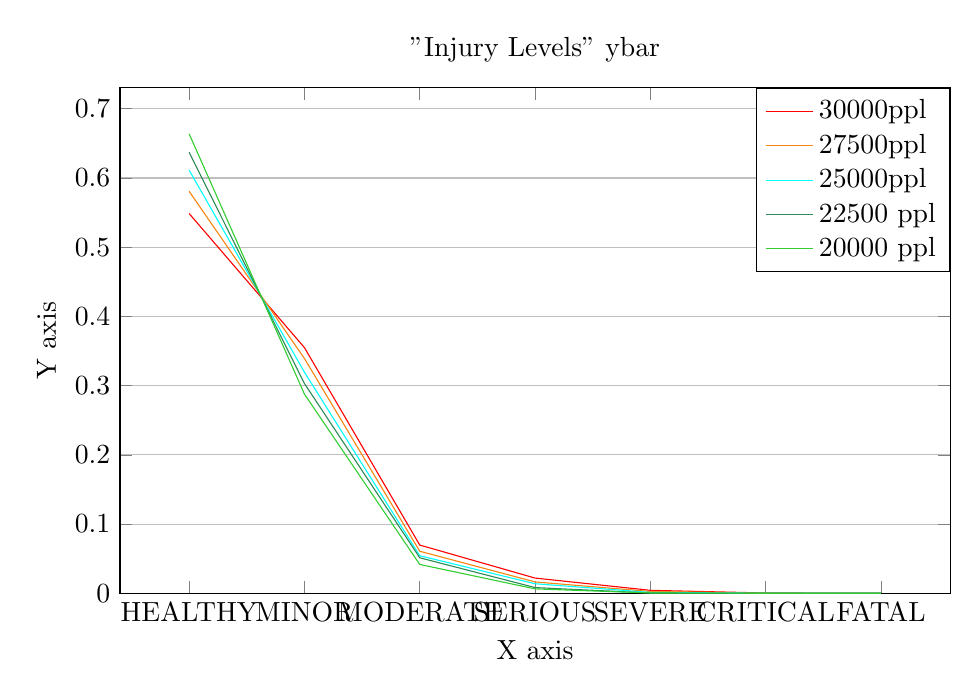
\begin{tikzpicture}
\begin{axis}[
title="Injury Levels"
ybar, % style of the histogram: clustered columns
width=\textwidth, % width of the plot
height=8cm, % height of the plot
xlabel={X axis}, % label for the x-axis
ylabel={Y axis}, % label for the y-axis
symbolic x coords={HEALTHY,MINOR,MODERATE,SERIOUS,SEVERE,CRITICAL,FATAL}, % labels for the x-ticks
xtick=data, % position the x-ticks at the data points
ymin=0, % minimum value of the y-axis
legend style={at={(1,1)}, anchor=north east}, % position of the legend
legend cell align=left, % alignment of the legend cells
ymajorgrids=true, % display major grids
bar width=0.25cm % width of the bars
]
\addplot[color=Red] coordinates{(HEALTHY,0.5486333333333333)(MINOR,0.3549333333333333)(MODERATE,0.06966666666666667)(SERIOUS,0.021966666666666666)(SEVERE,0.004266666666666667)(CRITICAL,0.0004)(FATAL,0.00013333333333333334)
}; % plot of the first histogram
\addplot[color=BurntOrange] coordinates{(HEALTHY,0.5807636363636364)(MINOR,0.3391636363636364)(MODERATE,0.06072727272727273)(SERIOUS,0.0164)(SEVERE,0.002618181818181818)(CRITICAL,0.00025454545454545456)(FATAL,7.272727272727273e-05)
}; % plot of the second histogram
\addplot[color=Cyan] coordinates{(HEALTHY,0.61132)(MINOR,0.31936)(MODERATE,0.0542)(SERIOUS,0.01376)(SEVERE,0.00128)(CRITICAL,8e-05)(FATAL,0.0)
}; % plot of the third histogram
\addplot[color=SeaGreen] coordinates{(HEALTHY,0.6370222222222223)(MINOR,0.30302222222222225)(MODERATE,0.05128888888888889)(SERIOUS,0.008222222222222223)(SEVERE,0.0004)(CRITICAL,4.4444444444444447e-05)(FATAL,0.0)
}; % plot of the fourth histogram
\addplot[color=LimeGreen] coordinates{(HEALTHY,0.6638)(MINOR,0.28775)(MODERATE,0.04165)(SERIOUS,0.00635)(SEVERE,0.0004)(CRITICAL,5e-05)(FATAL,0.0)
}; % plot of the fifth histogram
\legend{30000ppl,  27500ppl, 25000ppl, 22500 ppl, 20000 ppl} % legend of the plot
\end{axis}
\end{tikzpicture}
\end{document}